\chapter*{Introduction}\label{sec:introduction}
 The aim of this project is to study the behaviour of three different versions of the same application for Android devices through antimalware, static, and dynamic analysis.
 The main goal was to identify the malicious payload inside the APK files of the provided samples.

 The project is composed of three different files:
 \begin{enumerate}
     \item {\one}, (from now on it will be "\oner"), see Chapter \ref{one}
     \item \two, (from now on it will be "\twor"), see Chapter \ref{two}
     \item \three, (from now on it will be "\threer"), see Chapter \ref{three}
 \end{enumerate}

\section{Background: the Malbus Family}
\begin{figure}[h!]
    \centering
    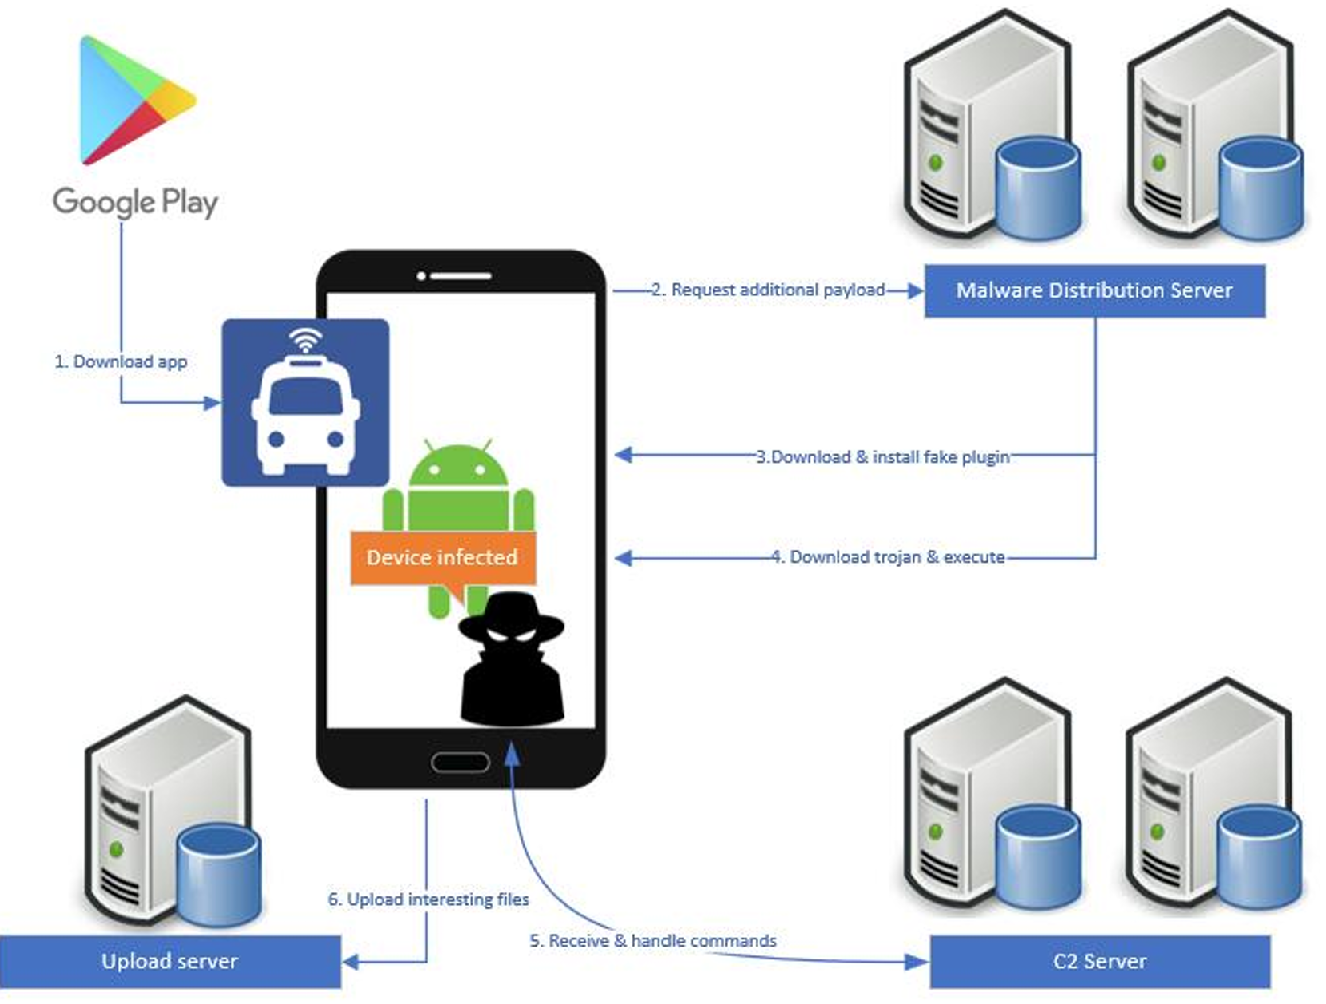
\includegraphics[width=.6\linewidth]{img/common/malbus_mcafee_chain.jpg}
    \caption{Malbus infection chain as documented by McAfee Mobile Research}
    \label{fig:malbus_mcafee_chain}
\end{figure}
The three samples analysed in this project belong to a malware family publicly documented by McAfee researchers under the name \textbf{Malbus}. The family was first described in a McAfee Mobile Research report detailing a series of trojanised Android applications masquerading as legitimate bus-information services targeting South Korean users. The malicious apps were distributed on the Google Play Store and, once installed, silently contacted remote servers to download and execute additional payloads on the victim device.

The McAfee-documented infection chain, illustrated in Fig.\ \ref{fig:malbus_mcafee_chain}, unfolds in six stages. The user first downloads the apparently legitimate bus app from Google Play (step~1). The app then contacts a Malware Distribution Server to request an additional payload (step~2), which is delivered and installed on the device as a fake plug-in (step~3). A second download delivers and executes the core trojan (step~4). From this point on, the infected device communicates bidirectionally with a Command-and-Control (C2) server to receive and handle commands (step~5), while a separate Upload Server is used to exfiltrate files of interest collected from the device (step~6).

The three APK samples provided for this project correspond to different versions of the same repackaged application series (\texttt{cwbus}, \texttt{gjbus}, \texttt{jjbus}), each targeting a different South Korean city. They represent successive releases of the Malbus dropper, allowing for a comparative analysis of how the malicious infrastructure and evasion techniques evolved across versions. The findings of the individual analyses are consolidated in Chapter~\ref{chap:comparison}.

\section{Tools}
  During the analysis, three main analysis tools have been used to identify malicious behaviour of the samples.
 \begin{itemize}
     \item VirusTotal \link{virustotal.com} (anti-malware analysis)
     \begin{itemize}
         \item It is a web tool that allows to submit samples and analyse them with several antivirus or anti-malware programmes
         \item This tool was used to gain an initial insight into the already existing knowledge about the specific malicious sample.
     \end{itemize}
     \item MobSF \link{github.com/MobSF/Mobile-Security-Framework-MobSF} (static and dynamic analysis)
 \begin{itemize}
     \item It automatically highlights interesting features of the application (e.g. Android permissions, API calls, remote URLs). It also extracts the Java code from the APK file. In this way we can gain a strong insight of the potential malicious behavior of the application and then manually analyze it by examining the code.
 \item Moreover, it performs a dynamic analysis, by executing the application inside a virtual environment and by monitoring it.
 \end{itemize}
 \item Java Decompiler \link{java-decompiler.github.io}
\begin{itemize}
    \item This tool allows users to displays Java source codes of ".class" files graphically. It can browse the reconstructed source code with the Java Decompiler Graphical User Interface (GUI) for instant access to methods and fields.
\end{itemize}
 \item Genymotion \link{genymotion.com} (dynamic analysis)
 \begin{itemize}

 \item Creates a virtual environment for MobSF in order to execute the malware sample safely.
 \end{itemize}
 \end{itemize}
